%!TEX program = xelatex
\documentclass[aspectratio=169]{ctexbeamer}
\usepackage[bluetheme]{ustcbeamer}
\input{ustctheme.tex}
\usepackage{booktabs}
\usepackage{graphicx}
\usepackage{array}
\usepackage{listings}

\lstset{
  language=Python,
  basicstyle=\ttfamily\scriptsize,
  breaklines=true,
  columns=fullflexible,
  frame=single,
  showstringspaces=false
}

\title[电商行为大数据分析]{基于电商用户行为大数据的消费转化漏斗与购买预测分析}
\author[期末大作业]{报告人：图力格尔}
\institute[USTC]{Python 经济大数据分析课程期末展示}
\date{\today}

\begin{document}

\maketitleframe

\begin{frame}
  \frametitle{大纲}
  \tableofcontents[hideallsubsections]
\end{frame}

\AtBeginSection[]{
\setbeamertemplate{footline}[footlineoff]
  \begin{frame}
    \frametitle{大纲}
    \tableofcontents[currentsection,subsectionstyle=show/show/hide]
  \end{frame}
\setbeamertemplate{footline}[footlineon]
}

\section{研究问题}

\begin{frame}
  \frametitle{为什么选择电商用户行为数据}
  \begin{itemize}
    \item 电商平台记录了用户从浏览、加购到购买的完整消费路径。
    \item 用户行为日志天然具有经济含义：消费意愿、促销响应、品类偏好、品牌选择。
    \item 原始数据达到亿级记录，适合展示 Python 分块处理、聚合分析和机器学习建模。
    \item 研究目标不是只画统计图，而是回答“哪里流失、什么卖得好、谁更可能购买”。
  \end{itemize}
\end{frame}

\begin{frame}
  \frametitle{核心研究问题}
  \begin{enumerate}
    \item 三个月内浏览、加购、购买的总体行为结构如何？
    \item 10 月、11 月、12 月之间是否存在促销季和年末消费差异？
    \item 哪些品类、品牌和价格区间贡献了主要交易额？
    \item 能否利用用户行为特征预测其是否发生购买？
  \end{enumerate}
\end{frame}

\section{数据与方法}

\begin{frame}
  \frametitle{指标体系}
  \begin{table}
  \centering
  \begin{tabular}{p{0.20\textwidth}p{0.32\textwidth}p{0.36\textwidth}}
  \toprule
  层面 & 指标 & 作用 \\
  \midrule
  规模 & 浏览、加购、购买、金额 & 衡量平台整体活跃和交易规模 \\
  转化 & 浏览到加购、浏览到购买、加购到购买 & 判断用户在哪个环节流失 \\
  结构 & 品类、品牌、价格区间 & 找到主要交易来源 \\
  预测 & Precision、Recall、F1、特征系数 & 识别潜在购买用户 \\
  \bottomrule
  \end{tabular}
  \end{table}
\end{frame}

\begin{frame}
  \frametitle{数据来源与规模}
  \begin{table}
  \centering
  \begin{tabular}{lr}
  \toprule
  项目 & 数值 \\
  \midrule
  数据来源 & Kaggle 电商行为数据集 \\
  时间范围 & 2019-10 至 2019-12 \\
  文件形态 & csv.gz / csv.zip \\
  总记录数 & 177,493,621 \\
  分块大小 & 每块 1,000,000 行 \\
  本地处理耗时 & 约 22.7 分钟 \\
  \bottomrule
  \end{tabular}
  \end{table}
\end{frame}

\begin{frame}
  \frametitle{数据口径：事件与用户分开处理}
  \begin{itemize}
    \item 事件口径：直接统计每条日志，用于浏览量、加购量、购买量和销售额。
    \item 用户口径：对 user\_id 去重，用于漏斗和用户购买倾向识别。
    \item 全量事件统计保留 1.77 亿条日志的信息。
    \item 唯一用户漏斗采用 user\_id 固定取模抽样估计，避免本地内存压力。
    \item 报告中明确区分“事件数”和“估计唯一用户数”，避免口径混用。
  \end{itemize}
\end{frame}

\begin{frame}
  \frametitle{分析流程}
  \begin{columns}
    \begin{column}{0.48\textwidth}
      \begin{block}{数据处理}
      \begin{itemize}
        \item 压缩 CSV 分块读取
        \item 时间、价格、品类、品牌清洗
        \item 日、月、小时维度聚合
        \item 品类、品牌、价格区间统计
      \end{itemize}
      \end{block}
    \end{column}
    \begin{column}{0.48\textwidth}
      \begin{block}{建模分析}
      \begin{itemize}
        \item 用户-月份特征表
        \item 确定性用户抽样
        \item 逻辑回归购买预测
        \item 混淆矩阵与特征解释
      \end{itemize}
      \end{block}
    \end{column}
  \end{columns}
\end{frame}

\begin{frame}[fragile]
  \frametitle{分块处理的核心实现}
  \begin{lstlisting}
reader = pd.read_csv(file_path, usecols=usecols,
                     chunksize=1_000_000,
                     compression="infer")

for chunk in reader:
    chunk["event_time"] = pd.to_datetime(
        chunk["event_time"], utc=True, errors="coerce"
    )
    chunk["month"] = chunk["event_time"].dt.strftime("%Y-%m")
    chunk["is_purchase"] = (chunk["event_type"] == "purchase")
  \end{lstlisting}
  \vspace{0.2cm}
  每次只处理 100 万行，保留聚合结果和用户抽样特征，不长期保存原始明细。
\end{frame}

\section{行为结构}

\begin{frame}
  \frametitle{三个月行为事件总量}
  \begin{columns}
    \begin{column}{0.58\textwidth}
      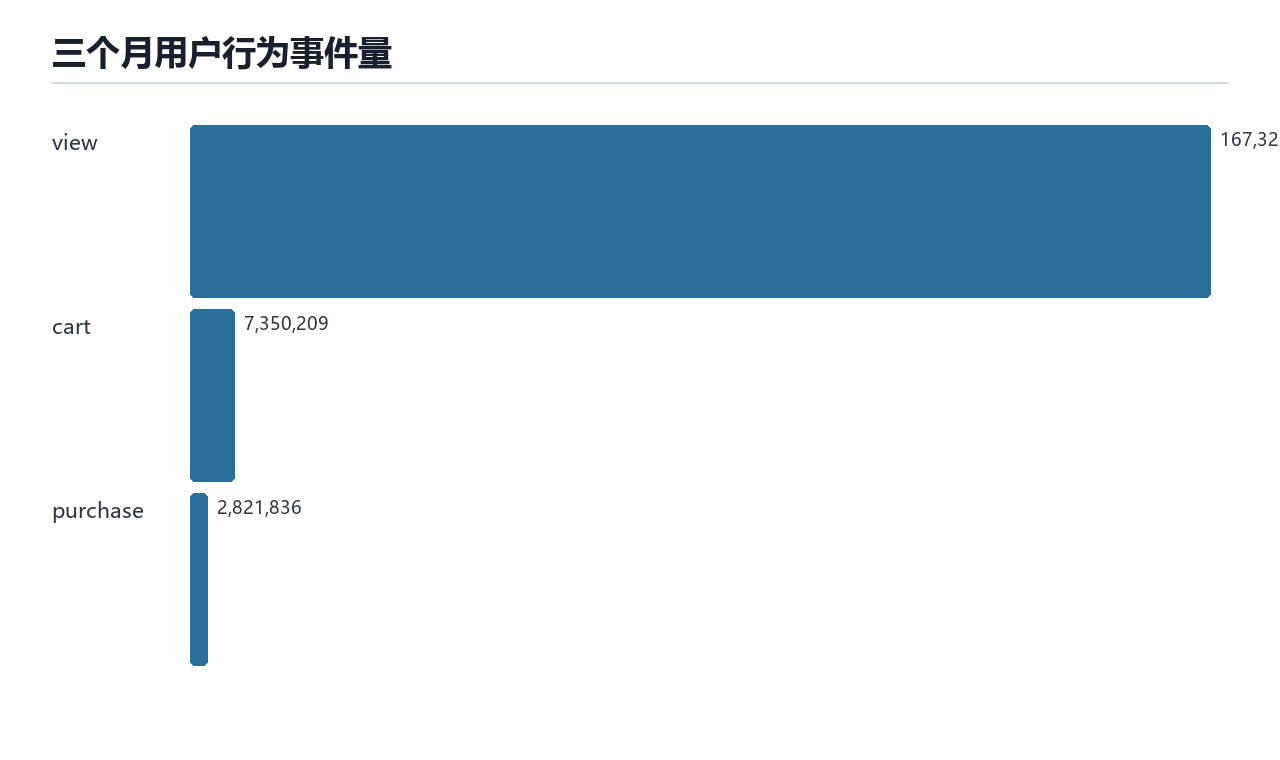
\includegraphics[width=\textwidth]{figures/event_type_summary.png}
    \end{column}
    \begin{column}{0.38\textwidth}
      \begin{itemize}
        \item 浏览：167,321,576 次
        \item 加购：7,350,209 次
        \item 购买：2,821,836 次
        \item 购买金额：849,329,221.91
      \end{itemize}
    \end{column}
  \end{columns}
\end{frame}

\begin{frame}
  \frametitle{月度行为对比}
  \begin{table}
  \centering
  \begin{tabular}{lrrr}
  \toprule
  月份 & 浏览 & 加购 & 购买 \\
  \midrule
  2019-10 & 40,779,399 & 926,516 & 742,849 \\
  2019-11 & 63,556,110 & 3,028,930 & 916,939 \\
  2019-12 & 62,986,067 & 3,394,763 & 1,162,048 \\
  \bottomrule
  \end{tabular}
  \end{table}
  \vspace{0.2cm}
  11 月和 12 月的流量与购买量明显高于 10 月，但流量增长并不自动等于转化效率提升。
\end{frame}

\begin{frame}
  \frametitle{小时维度：不同动作的峰值不同}
  \begin{table}
  \centering
  \begin{tabular}{lrr}
  \toprule
  行为 & 峰值小时 & 峰值事件数 \\
  \midrule
  浏览 & 16 点 & 11,564,432 \\
  加购 & 8 点 & 495,343 \\
  购买 & 9 点 & 211,140 \\
  \bottomrule
  \end{tabular}
  \end{table}
  \begin{itemize}
    \item 浏览更像信息搜索和比较。
    \item 加购与购买更接近明确消费动作。
    \item 推荐曝光、购物车提醒和支付激励可以分时段设计。
  \end{itemize}
\end{frame}

\begin{frame}
  \frametitle{日度行为变化}
  \centering
  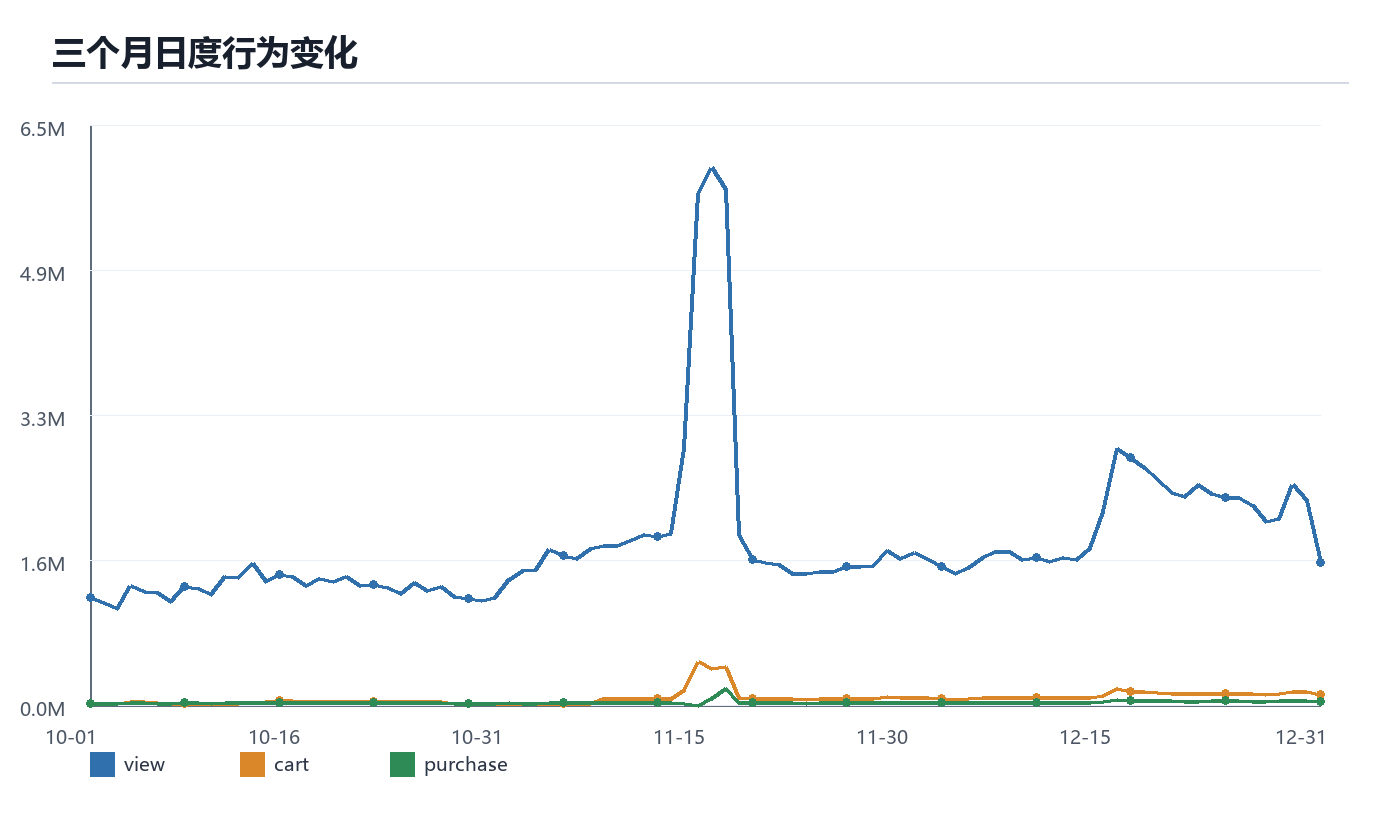
\includegraphics[width=0.94\textwidth]{figures/daily_events.png}
\end{frame}

\begin{frame}
  \frametitle{加购到购买转化率}
  \begin{columns}
    \begin{column}{0.58\textwidth}
      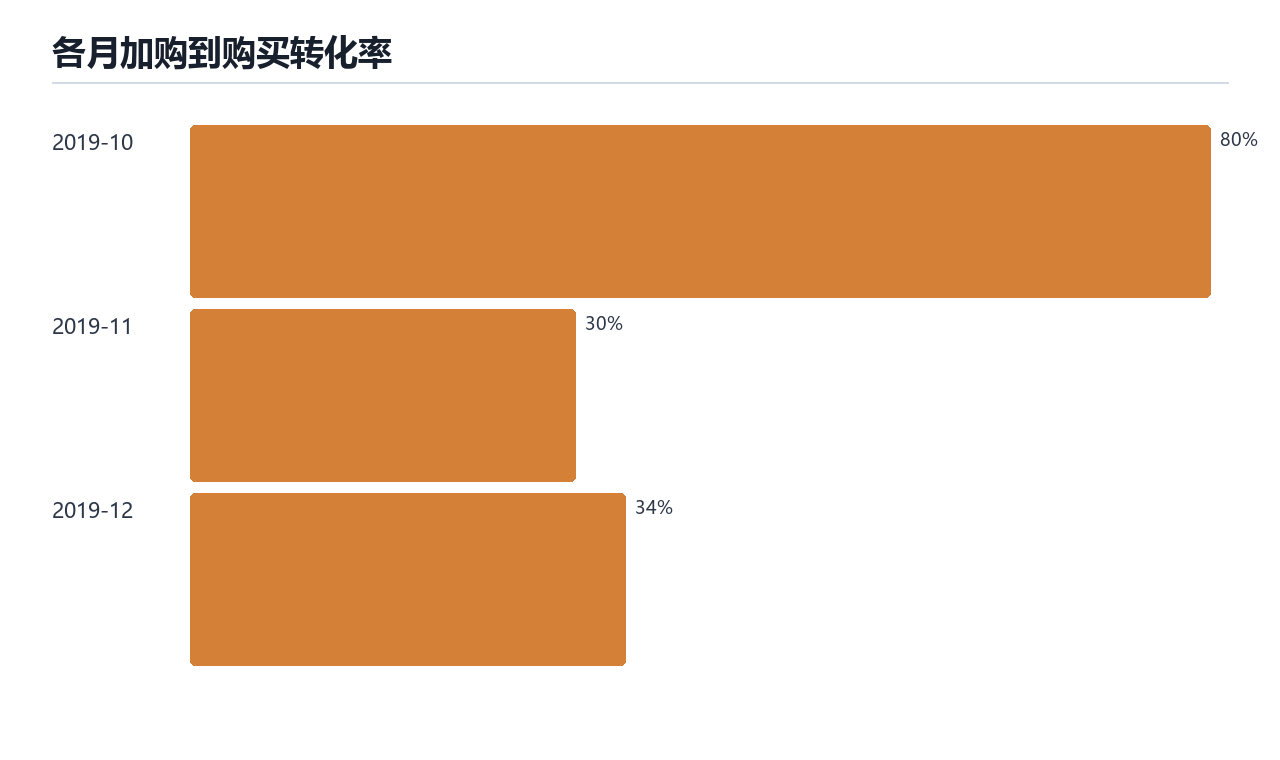
\includegraphics[width=\textwidth]{figures/monthly_cart_purchase_rate.png}
    \end{column}
    \begin{column}{0.38\textwidth}
      \begin{itemize}
        \item 10 月购买规模较小，但加购到购买比例较高。
        \item 11 月流量和加购明显放大，转化效率被摊薄。
        \item 12 月购买量继续上升，年末消费需求更强。
      \end{itemize}
    \end{column}
  \end{columns}
\end{frame}

\section{转化漏斗}

\begin{frame}
  \frametitle{用户转化漏斗}
  \begin{columns}
    \begin{column}{0.56\textwidth}
      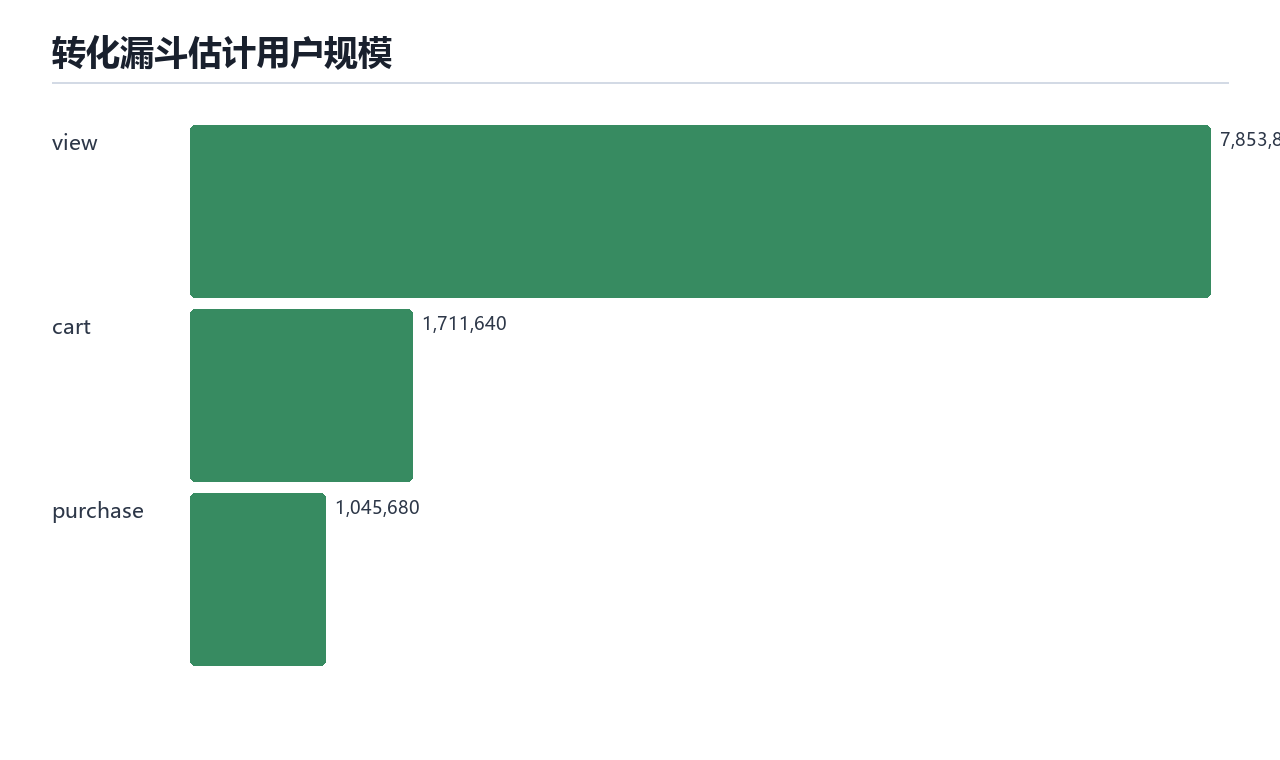
\includegraphics[width=\textwidth]{figures/funnel_users.png}
    \end{column}
    \begin{column}{0.40\textwidth}
      \begin{table}
      \centering
      \begin{tabular}{lrr}
      \toprule
      阶段 & 估计用户数 & 占比 \\
      \midrule
      浏览 & 7,853,880 & 100.00\% \\
      加购 & 1,711,640 & 21.79\% \\
      购买 & 1,045,680 & 13.31\% \\
      \bottomrule
      \end{tabular}
      \end{table}
    \end{column}
  \end{columns}
\end{frame}

\begin{frame}
  \frametitle{漏斗结果的业务含义}
  \begin{itemize}
    \item 浏览到加购：反映商品匹配、搜索推荐和详情页质量。
    \item 加购到购买：反映价格、促销、库存、配送和支付体验。
    \item 加购未购买用户已经表现出较强意向，是平台二次触达的重点对象。
    \item 促销期不应只看访问峰值，还要看购物车沉淀后的支付转化。
  \end{itemize}
\end{frame}

\section{品类与品牌}

\begin{frame}
  \frametitle{销售额最高的品类}
  \centering
  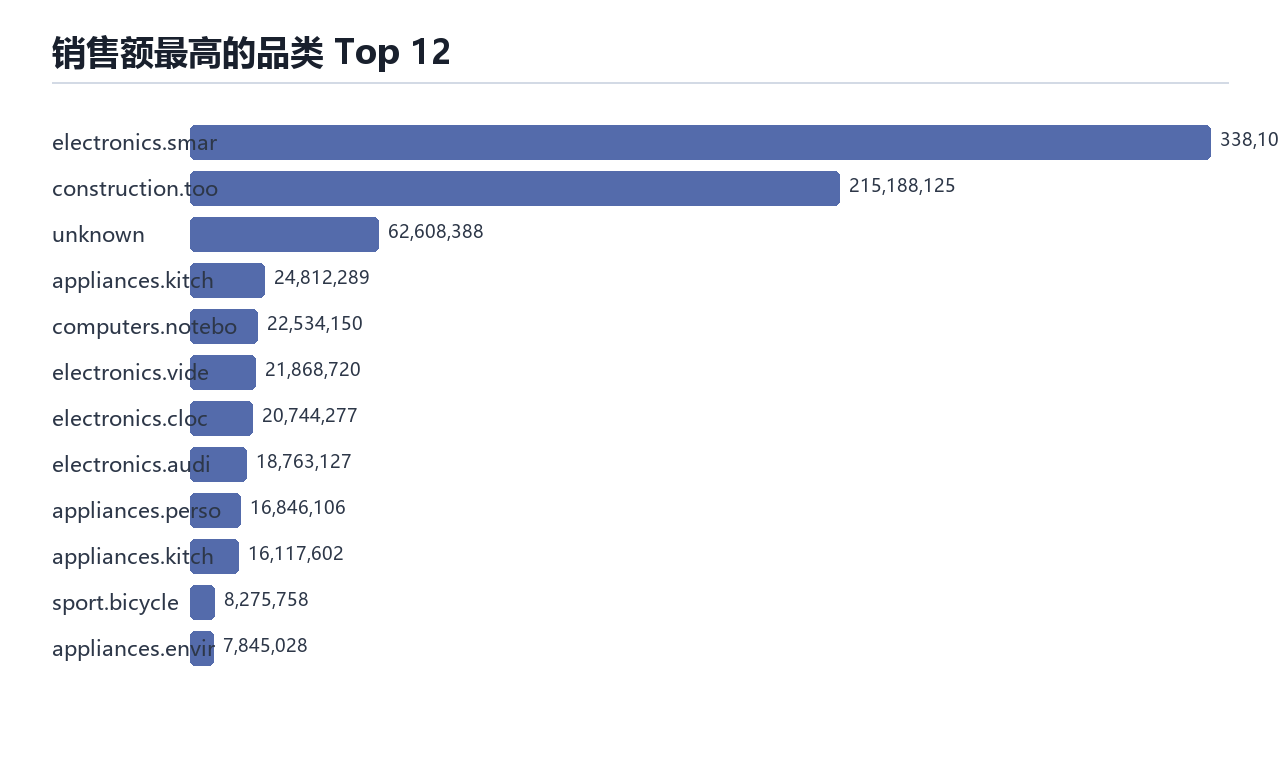
\includegraphics[width=0.92\textwidth]{figures/top_categories_revenue.png}
\end{frame}

\begin{frame}
  \frametitle{销售额最高的品牌}
  \centering
  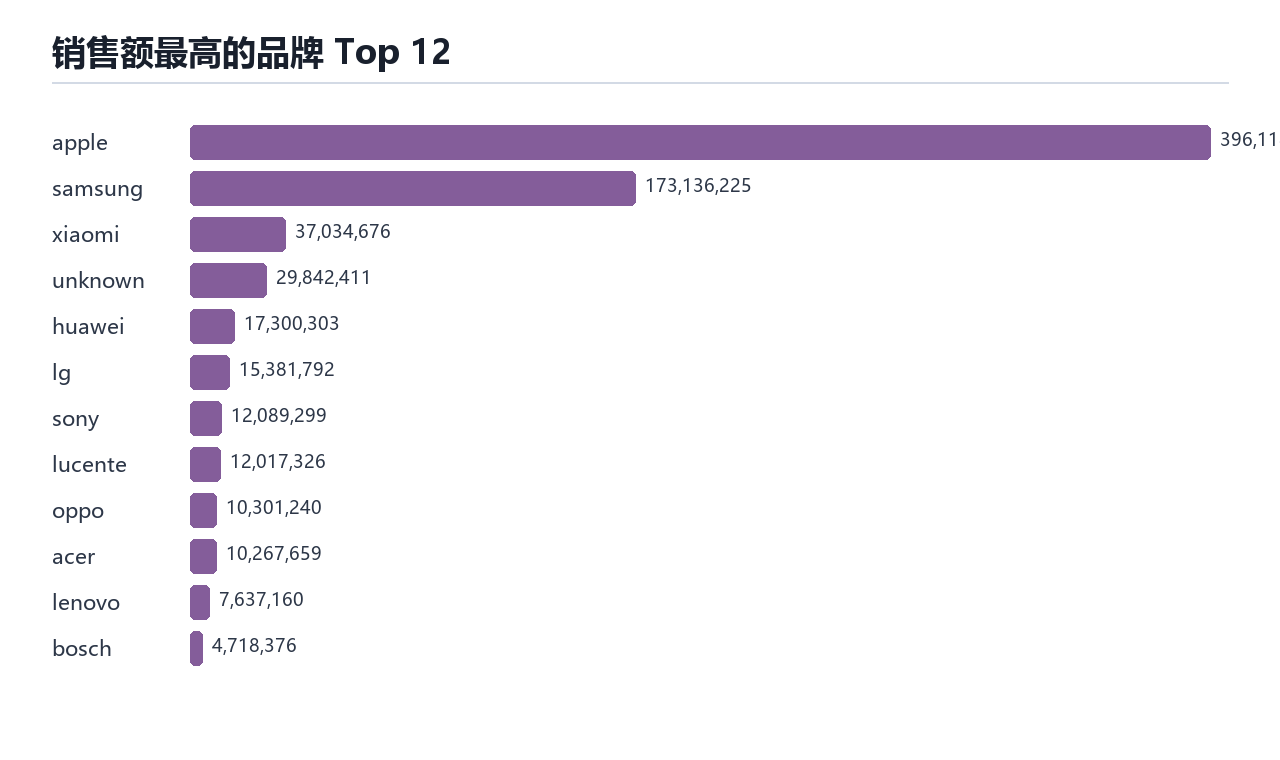
\includegraphics[width=0.92\textwidth]{figures/top_brands_revenue.png}
\end{frame}

\begin{frame}
  \frametitle{品类与品牌发现}
  \begin{itemize}
    \item 手机、灯具工具、耳机、钟表、电视和家电贡献主要交易额。
    \item Apple 购买次数低于 Samsung，但销售额更高，体现高客单价特征。
    \item Samsung 购买次数最高，说明其覆盖更广泛的交易需求。
    \item unknown 品类和品牌占比不低，实际业务中需要改进商品信息治理。
  \end{itemize}
\end{frame}

\begin{frame}
  \frametitle{价格带结构：交易频次与金额贡献不同}
  \begin{table}
  \centering
  \begin{tabular}{lrr}
  \toprule
  价格区间 & 购买金额 & 金额占比 \\
  \midrule
  500--1000 & 268,103,353.39 & 31.57\% \\
  200--500 & 233,270,380.69 & 27.47\% \\
  1000--5000 & 194,988,617.34 & 22.96\% \\
  100--200 & 113,879,642.68 & 13.41\% \\
  \bottomrule
  \end{tabular}
  \end{table}
  中低价商品贡献交易频次，高价商品贡献销售额，需要分别管理。
\end{frame}

\section{购买预测}

\begin{frame}
  \frametitle{机器学习任务设定}
  \begin{block}{预测目标}
    以用户-月份为样本，预测用户当月是否发生购买。
  \end{block}
  \begin{block}{输入特征}
    总行为次数、浏览次数、加购次数、会话数、活跃天数、浏览商品数、浏览品类数、浏览品牌数、平均价格、最高价格。
  \end{block}
  \begin{block}{模型}
    使用 NumPy 实现逻辑回归，并对正样本设置权重以缓解类别不平衡。
  \end{block}
\end{frame}

\begin{frame}
  \frametitle{标签口径：购买倾向识别，不夸大为实时预测}
  \begin{itemize}
    \item 样本单位：用户-月份。
    \item 标签：当月是否至少发生一次购买。
    \item 特征：当月行为强度、会话数、活跃天数、商品/品类/品牌范围、价格偏好。
    \item 当前模型适合识别高购买倾向用户。
    \item 更严格的实时预测应使用“前期行为预测后期购买”的时间切分。
  \end{itemize}
\end{frame}

\begin{frame}
  \frametitle{模型评估结果}
  \begin{columns}
    \begin{column}{0.48\textwidth}
      \begin{table}
      \centering
      \begin{tabular}{lr}
      \toprule
      指标 & 数值 \\
      \midrule
      测试集样本 & 50,000 \\
      正样本比例 & 11.43\% \\
      Accuracy & 89.95\% \\
      Precision & 53.68\% \\
      Recall & 85.49\% \\
      F1 & 0.659 \\
      \bottomrule
      \end{tabular}
      \end{table}
    \end{column}
    \begin{column}{0.48\textwidth}
      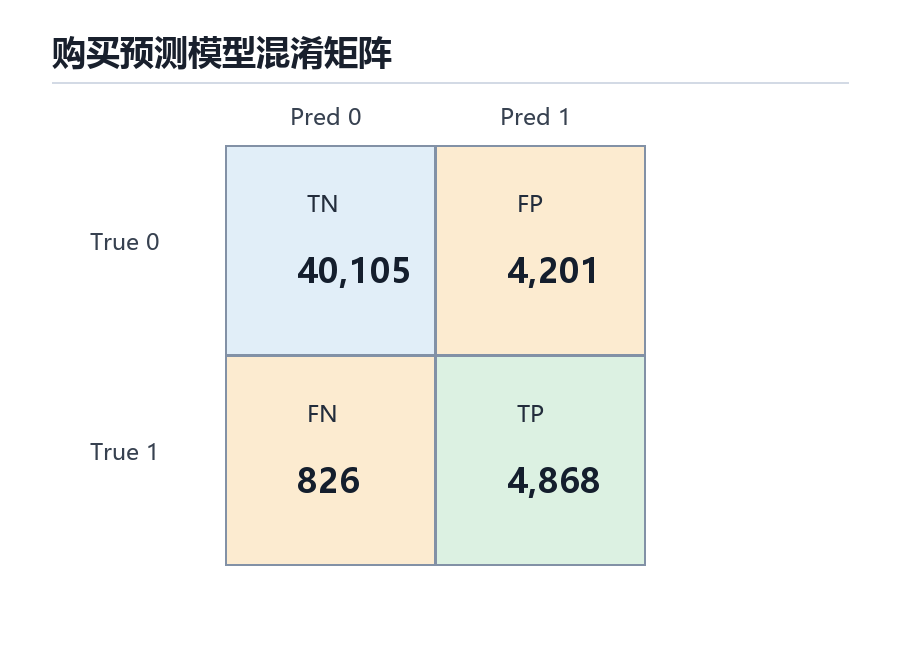
\includegraphics[width=\textwidth]{figures/model_confusion_matrix.png}
    \end{column}
  \end{columns}
\end{frame}

\begin{frame}
  \frametitle{特征重要性}
  \begin{columns}
    \begin{column}{0.58\textwidth}
      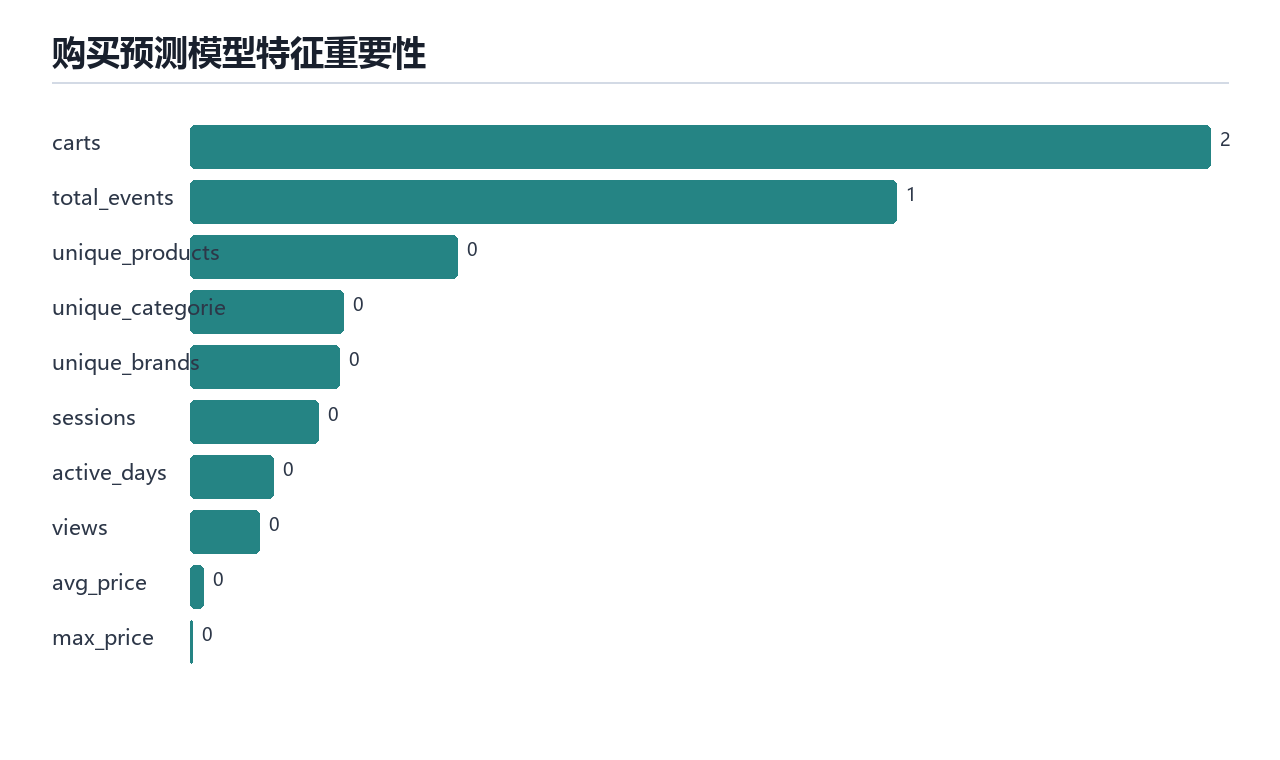
\includegraphics[width=\textwidth]{figures/model_feature_importance.png}
    \end{column}
    \begin{column}{0.38\textwidth}
      \begin{itemize}
        \item 加购次数是最强购买意图信号。
        \item 总行为次数和会话数反映用户活跃程度。
        \item 浏览范围过宽可能意味着仍在比较，购买确定性下降。
      \end{itemize}
    \end{column}
  \end{columns}
\end{frame}

\begin{frame}
  \frametitle{从模型结果到运营动作}
  \begin{table}
  \centering
  \begin{tabular}{p{0.30\textwidth}p{0.55\textwidth}}
  \toprule
  用户信号 & 可采取动作 \\
  \midrule
  多次加购未购买 & 库存提醒、支付提醒、必要时价格激励 \\
  浏览范围广但未加购 & 强化筛选、推荐排序、商品对比信息 \\
  高价商品浏览用户 & 突出售后、品牌信任、分期和保障服务 \\
  购买倾向模型名单 & 用作营销触达人群池，再按预算排序 \\
  \bottomrule
  \end{tabular}
  \end{table}
\end{frame}

\section{购物车转化深化}

\begin{frame}
  \frametitle{为什么进一步聚焦加购后转化}
  \begin{itemize}
    \item 原用户-月份模型适合识别购买倾向，但不是严格实时预测。
    \item 漏斗中最有业务价值的一段是 cart-to-purchase。
    \item 当前数据集正好包含 view、cart、purchase 行为链路。
    \item 新任务：首次加购前/加购时可见信息，预测后续是否购买。
    \item 这比“当月行为预测当月购买”更能避免时间口径问题。
  \end{itemize}
\end{frame}

\begin{frame}
  \frametitle{样本与标签定义}
  \begin{table}
  \centering
  \begin{tabular}{p{0.26\textwidth}p{0.58\textwidth}}
  \toprule
  项目 & 定义 \\
  \midrule
  样本单位 & user\_session \\
  入样条件 & session 内至少出现一次 cart \\
  观察点 & session 的首次 cart 时刻 \\
  主标签 & 首次 cart 后，session 内是否发生任意 purchase \\
  辅助标签 & 首次 cart 的商品后续是否被 purchase \\
  划分方式 & 10--11 月训练，12 月测试 \\
  \bottomrule
  \end{tabular}
  \end{table}
\end{frame}

\begin{frame}
  \frametitle{工程实现：跨 chunk 的 session 状态}
  \begin{itemize}
    \item 扫描三个月全量 177,493,621 条日志。
    \item 按 user\_id 进行 1/20 确定性抽样，处理 8,879,159 条行为。
    \item 维护 session\_state 字典，不保存原始明细。
    \item 每个 session 只保留首次 cart 前统计、首次 cart 信息和后续购买标签。
    \item 最终得到 216,713 个加购 session 样本，样本构造耗时约 7.76 分钟。
  \end{itemize}
\end{frame}

\begin{frame}
  \frametitle{购物车转化模型结果}
  \begin{columns}
    \begin{column}{0.50\textwidth}
      \begin{table}
      \centering
      \begin{tabular}{lr}
      \toprule
      指标 & 数值 \\
      \midrule
      12 月测试样本 & 99,323 \\
      测试集购买率 & 48.12\% \\
      Precision & 48.67\% \\
      Recall & 97.13\% \\
      F1 & 0.648 \\
      \bottomrule
      \end{tabular}
      \end{table}
    \end{column}
    \begin{column}{0.46\textwidth}
      \begin{itemize}
        \item 分类阈值不是核心。
        \item 更重要的是高意向 session 的排序能力。
        \item 因此重点看 TopK 和 Lift。
      \end{itemize}
    \end{column}
  \end{columns}
\end{frame}

\begin{frame}
  \frametitle{TopK/Lift：更贴近营销排序}
  \begin{columns}
    \begin{column}{0.54\textwidth}
      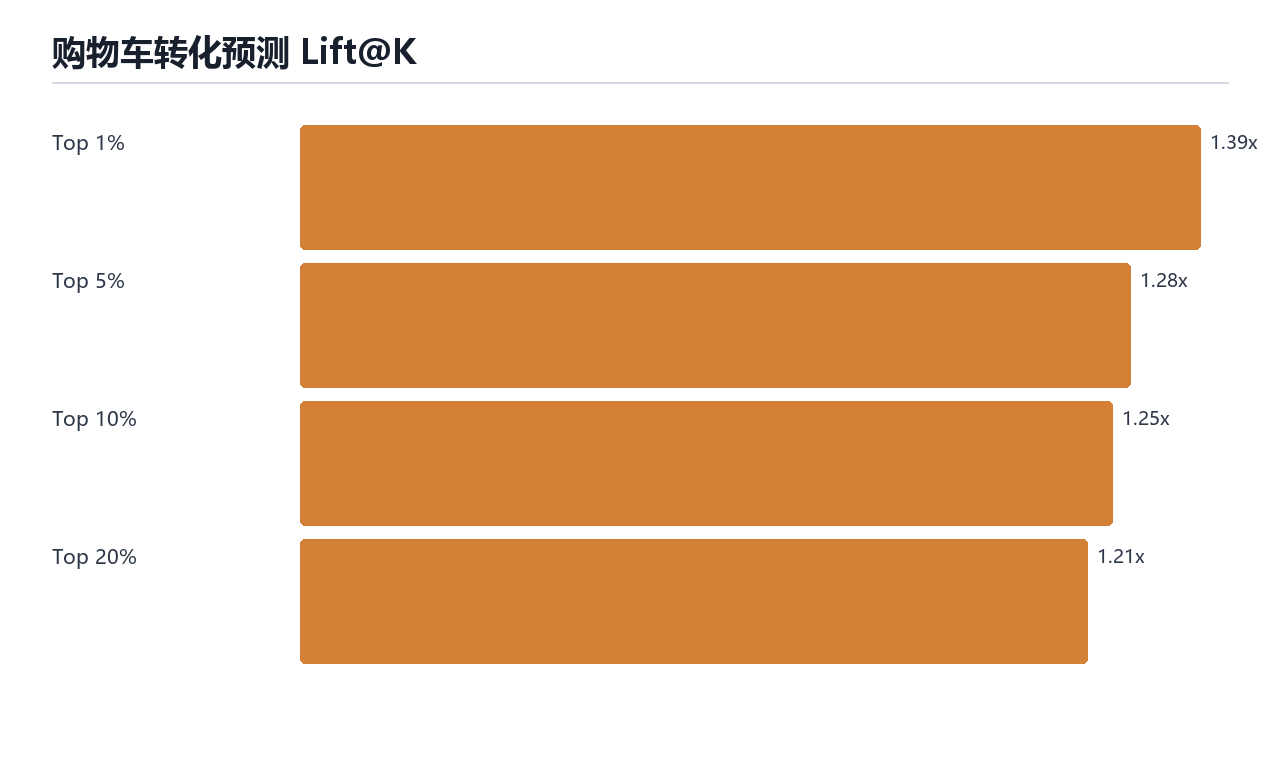
\includegraphics[width=\textwidth]{figures/cart_conversion_lift.png}
    \end{column}
    \begin{column}{0.42\textwidth}
      \begin{table}
      \centering
      \begin{tabular}{lrr}
      \toprule
      用户池 & Precision & Lift \\
      \midrule
      Top 1\% & 66.67\% & 1.39 \\
      Top 5\% & 61.54\% & 1.28 \\
      Top 10\% & 60.22\% & 1.25 \\
      Top 20\% & 58.31\% & 1.21 \\
      \bottomrule
      \end{tabular}
      \end{table}
    \end{column}
  \end{columns}
\end{frame}

\begin{frame}
  \frametitle{购物车转化模型特征}
  \begin{columns}
    \begin{column}{0.56\textwidth}
      
\includegraphics[width=\textwidth]{figures/cart_conversion_feature_importance.png}
    \end{column}
    \begin{column}{0.40\textwidth}
      \begin{itemize}
        \item 首次 cart 前 session 持续时间影响最大。
        \item 首次加购价格和浏览商品范围提供额外信号。
        \item 加购小时、商品此前浏览次数也能帮助排序。
      \end{itemize}
    \end{column}
  \end{columns}
\end{frame}

\begin{frame}
  \frametitle{业务解释边界}
  \begin{itemize}
    \item 高预测分数表示更可能自然购买，不等于最需要发券。
    \item 高自然转化用户：适合库存提醒、支付提醒、服务保障。
    \item 低自然转化但高价格 session：更接近召回候选池。
    \item 本文识别到 5,545 个“低自然转化概率 + 高加购价格”session。
    \item 数据没有优惠券、曝光、库存和物流字段，因此不做促销因果解释。
  \end{itemize}
\end{frame}

\section{结论}

\begin{frame}
  \frametitle{主要结论}
  \begin{enumerate}
    \item 三个月 1.77 亿条日志呈现明显浏览、加购、购买漏斗。
    \item 11 月和 12 月行为规模较大，但转化效率需要单独监控。
    \item 消费电子和家电相关品类贡献主要销售额。
    \item 月度模型识别购买倾向，购物车模型进一步预测首次加购后的 session 转化。
    \item 购物车转化模型 Top 10\% 高分 session 真实购买率为 60.22\%，Lift 为 1.25。
  \end{enumerate}
\end{frame}

\begin{frame}
  \frametitle{运营建议与不足}
  \begin{columns}
    \begin{column}{0.48\textwidth}
      \begin{block}{建议}
      \begin{itemize}
        \item 对加购未购买用户重点触达
        \item 促销期同时关注流量和支付转化
        \item 对高销售额品类优化库存和价格带
      \end{itemize}
      \end{block}
    \end{column}
    \begin{column}{0.48\textwidth}
      \begin{block}{不足}
      \begin{itemize}
        \item 唯一用户漏斗采用抽样估计
        \item 模型尚未严格拆分购买前后行为
        \item 后续可尝试树模型和序列模型
      \end{itemize}
      \end{block}
    \end{column}
  \end{columns}
\end{frame}

\begin{frame}
  \frametitle{课程技术闭环}
  \begin{itemize}
    \item Python 脚本化：从原始压缩文件到图表和模型结果可复现。
    \item Pandas：分块读取、清洗、分组、透视和特征聚合。
    \item NumPy：逻辑回归的矩阵计算和评价指标计算。
    \item 可视化：将亿级日志压缩为行为漏斗、时间变化和结构图。
    \item 机器学习：将描述性分析推进到潜在购买用户识别。
  \end{itemize}
\end{frame}

\begin{frame}
  \frametitle{致谢}
  \centerline{\Large 谢谢!}
\end{frame}

\end{document}
